\documentclass[a4paper,11pt]{article}

\usepackage[utf8]{inputenc}
\usepackage[a4paper, left=3cm, right=3cm, top=3cm, bottom=3cm]{geometry}
\usepackage[frenchb]{babel}
\usepackage{default}
\usepackage{pslatex}
\usepackage{graphicx}
\usepackage{algorithmic}
\usepackage{multicol}
\usepackage{amsmath}
\usepackage{amssymb}
\usepackage{textcomp}
\usepackage{pgf}
\usepackage{tikz}
\usepackage{pgfplots}
\usepackage{capt-of}
\usepackage{esvect}
\usepackage[T1]{fontenc}
\usepackage[babel=true]{csquotes}

% \setcounter{tocdepth}{4}

%opening
\title{Tropodrone}
\author{Thibaut Manceau, Alexis Gros, Noé Gueydan, Tristan Porteries}

\begin{document}

\begin{Huge}
\maketitle
\end{Huge}

\clearpage

\tableofcontents

\clearpage

\section{Introduction}

\subsection{Besoins}

\subsection{Applications}

\subsection{Contraintes}

\subsubsection{Légalité}

\subsubsection{Drone}


\section{Étude de conception}

\subsection{Ballon}

\subsubsection{Élévation}

Le tropodrone doit utiliser un moyen de supporter une partie du poids du drone sans dépenser d'énérgie dans le but d'augmenter l'autonomie, pour ce faire nous utilisons la poussée d'Archimède d'un gaz plus léger que l'air. Comme ce gaz est plus léger que l'air la somme de son poids et de sa poussée d'Archimède forment une force verticale orienté vers le haut.

\paragraph{Archimède}

La poussée d'archimède est définie par~:

\enquote{Tout corps plongé dans un fluide au repos, entièrement mouillé par celui-ci ou traversant sa surface libre, subit une force verticale, dirigée de bas en haut et opposée au poids du volume de fluide déplacé ; cette force est appelée poussée d'Archimède.}

\begin{center}
	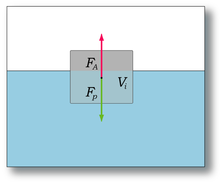
\includegraphics[width=5cm]{../Images/pousse_archimede.png}
\end{center}

Cette force se calcule avec la formule~:

\begin{center}
  \boxed{\vv{Fa} = -M_F \times \vv{g}}
\end{center}

Où $\vv{Fa}$ est la poussée d'archimède, $M_F$ la masse du fluide contenue dans le volume déplacé, $\vv{g}$ la valeur du champ de pesanteur. \\

Un ballon de gaz est donc soumis à deux forces~: son poids et sa poussée d'Archimède~:

\begin{center}
  \boxed{\vv{F_{ballon}} = \vv{P_{ballon}} + \vv{Fa_{ballon}}}
\end{center}

Où $\vv{F_{ballon}}$ est la force d'élévation du ballon, $\vv{P_{ballon}}$ le poids du ballon, $\vv{Fa_{ballon}}$ la poussée d'Archimède éxercée sur le ballon. \\

Nous pouvons remarquer que si $P_{ballon} < Fa_{ballon}$ alors il existe une force d'élévation orienté vers le haut. De même cette force sera toujours  plus petite que la poussée d'Archimède éxercée sur le ballon, comme le ballon et le gaz possède toujours une masse~: $F_{ballon} < Fa_{ballon}$.
Par la suite on appellera capacité d'élevation la masse que peut supporter la force d'élévation d'un ballon~:
\begin{center}
	\boxed{Ca_{ballon} = \frac{F_{ballon}}{g}}
\end{center}

Où $Ca_{ballon}$ est la capacité d'élévation, $F_{ballon}$ la force d'élévation et $g$ la valeur du champ de pesanteur.

\paragraph{Gaz}

Pour avoir un gaz plus léger que l'air il faut qu'il est une masse volumique inférieur à celle de l'air~: $1.29kg.m^3$. Plusieurs gazs remplissent cette condition, les plus courants sont l'hélium est l'hydrogène dont les masse volumique et les capacités d'élévation calculées sont~:

\begin{center}
	\begin{tabular}{|l|c|c|c|}
		\hline
		Gaz & Air & Hydrogène & Hélium \\
		\hline
		Masse Volumique $(kg.m^3)$ & 1.29 & 0.08988 & 0.1785 \\
		\hline
		Force d'élévation $(N.m^3)$ & 0 & 11.77 & 10.90 \\
		\hline
	\end{tabular}
\end{center}

\paragraph{Dilatation}

\subsubsection{Enveloppe}

\paragraph{Materiaux}

\paragraph{Étanchéité}

\subsubsection{Collage}

\paragraph{Résistance}

\subsection{Structure}

\subsubsection{Étude des mouvements}

\subsubsection{Support ballon}

\subsection{Support drone}

\paragraph{1er modèle}

\paragraph{2ème modèle}


\section{Aérodynamisme}

\subsection{Influence sur la structure}

\subsubsection{Optimisation avec la forme en triangle}

\subsubsection{Gouvernail}

\subsection{Équation de trainée}

\subsubsection{Calcul du Cx}

\paragraph{Simulation SW}
!= conformations

\subsection{Simulation Python}


\section{Réalisation}

\end{document}
